\section{6. Simulating the sensor values (the physical model)}

BuildSim provides the rooms but nothing that changes, so the fire, the air in every
room, the sensors and the people are all simulated here. The aim was never physical
fidelity. It was a model with enough structure that a decision made on its readings
means something: fires that keep growing, nuisances that peak and fade, smoke that
leaves through doors and climbs stairwells, and, above all, actuator commands that
change the next reading so that the loop closes.

\textbf{Sources.} A source is a scripted event with a kind, a room and a start
time. The kind is also the ground-truth label the scoreboard uses, and nothing
downstream of the sensors may read it. Each kind declares what it emits at time $e$
since ignition, as a heat release rate and the smoke and CO the room would settle
to if nothing else happened:

\begin{longtable}[]{@{}
  >{\raggedright\arraybackslash}p{(\columnwidth - 6\tabcolsep) * \real{0.16}}
  >{\raggedright\arraybackslash}p{(\columnwidth - 6\tabcolsep) * \real{0.16}}
  >{\raggedright\arraybackslash}p{(\columnwidth - 6\tabcolsep) * \real{0.34}}
  >{\raggedright\arraybackslash}p{(\columnwidth - 6\tabcolsep) * \real{0.34}}@{}}
\toprule
\textbf{Kind} & \textbf{Label} & \textbf{Emission} & \textbf{What makes it hard} \\
\midrule
\endhead
flaming & fire & $q = \min(\alpha e^2, q_{\max})$ with the standard $t^2$ growth coefficients (slow 0.0029 to ultrafast 0.1876\,kW/s$^2$); smoke $0.06\sqrt{q}$, CO $4\sqrt{q}$ & The easy case: everything corroborates \\
smouldering & fire & 3\,kW, smoke 0.9\,1/m and CO 900\,ppm, all ramping with $1-e^{-e/300}$ & Almost no heat, so the sprinkler interlock refuses water \\
cooking & nuisance & 12\,kW, smoke 0.35, CO 25\,ppm, as a bump that rises over 3\,min and fades over 15 & Warm and smoky, but the CO never comes \\
dust & nuisance & smoke 0.5, a 20\,s bump; no heat, no CO & Fools a smoke detector on its own \\
steam & nuisance & smoke 0.7, a 30\,s bump; no heat, no CO & As dust, denser and shorter \\
\bottomrule
\end{longtable}

The shape over time is what matters. A real fire keeps getting worse; a nuisance grows, holds
and fades. That difference over time, together with the ratio of CO to smoke, is
what the detector has to pick up.

\textbf{Room physics.} Every space is one lumped node with a true temperature
$T$, smoke obscuration $S$ and CO concentration $C$. Each step of $\Delta t$ seconds
has two phases. First each room relaxes towards where its own source is pushing it:
\[
  T \leftarrow T^{\ast} + (T - T^{\ast})\,e^{-\Delta t/\tau_T}, \qquad
  T^{\ast} = T_{\text{out}} + \min\!\Big(140\,\big(q/V\big)^{2/3},\; 900\Big),
\]
with the same first-order approach for smoke and CO towards their equilibrium
values, and time constants $\tau_T = 90$\,s, $\tau_S = 45$\,s, $\tau_C = 60$\,s.
$V$ is the room's volume, its floor area from the plan times a 3\,m ceiling, so a
lecture theatre dilutes a fire and a cupboard does not, and the sub-linear rise
with heat density is capped at post-flashover temperatures. Then neighbouring rooms
trade what they hold through every doorway and stairwell:
\[
  \Delta X_{a \to b} = \min\!\big(g\,k_X\,\Delta t,\; 0.5\big)\,(X_a - X_b),
  \qquad g = \text{conductance} \times \text{openness},
\]
for $X \in \{T, S, C\}$ with diffusion rates $k_S = 0.35$, $k_C = 0.30$,
$k_T = 0.12$. The conductance of a doorway comes from BuildSim's walkable graph and
is 0.6 for a stairwell, which is how smoke climbs floors. The share a room gives away
in one step is capped across all of its doorways together, because a corridor with
twenty doors would otherwise hand out several times what it holds and the building
would fill with smoke nobody produced. That was a real bug, found by running the
building at high speed.

\textbf{Closing the loop.} Two actuator states live inside the physics. An active
sprinkler multiplies the room's heat release by 0.25 and its smoke equilibrium by
0.4. A closed fire door sets the openness of every coupling into that room to
0.15, because a real fire door leaks. Both are written by the actuation zone and
read by the next physics step, so a command issued at tick $n$ changes the reading
at tick $n+1$. Section~11 measures what that buys.

\textbf{Sensors.} A reading is never the truth. Every device applies the same
chain, in this order, each step with its own per-modality parameters:

\begin{center}
\code{lag → calibration bias → noise → quantisation → clamp → fault}
\end{center}

\begin{longtable}[]{@{}
  >{\raggedright\arraybackslash}p{(\columnwidth - 12\tabcolsep) * \real{0.16}}
  >{\raggedright\arraybackslash}p{(\columnwidth - 12\tabcolsep) * \real{0.14}}
  >{\raggedright\arraybackslash}p{(\columnwidth - 12\tabcolsep) * \real{0.14}}
  >{\raggedright\arraybackslash}p{(\columnwidth - 12\tabcolsep) * \real{0.14}}
  >{\raggedright\arraybackslash}p{(\columnwidth - 12\tabcolsep) * \real{0.14}}
  >{\raggedright\arraybackslash}p{(\columnwidth - 12\tabcolsep) * \real{0.14}}
  >{\raggedright\arraybackslash}p{(\columnwidth - 12\tabcolsep) * \real{0.14}}@{}}
\toprule
\textbf{Modality} & \textbf{Lag $\tau$} & \textbf{Noise $\sigma$} & \textbf{Quantum} & \textbf{Range} & \textbf{Interval} & \textbf{Unit} \\
\midrule
\endhead
smoke & 12\,s & 0.010 & 0.005 & 0--3 & 5\,s & 1/m \\
CO & 25\,s & 3.0 & 1 & 0--2000 & 5\,s & ppm \\
temperature & 30\,s & 0.15 & 0.1 & $-20$--250 & 5\,s & °C \\
\bottomrule
\end{longtable}

Temperature lags most because a heat detector has thermal mass. The clamp at
250\,°C is why the dashboard shows a reading of 250 against a truth of 648 in a
developed fire: the detector is saturated, as a real one would be. Noise is scaled
by one live setting, 0 for a perfect instrument and 3 for a badly behaved one, and
the evaluation sweeps it. A device can also be given one of four faults: \emph{stuck}
repeats its last value, \emph{dropout} skips 40\,\% of samples, \emph{drift} adds an
error that grows without bound, and \emph{dead} reports nothing at all. Faults are
injected from the Rooms table and are what the two hardest presets are built on.

\textbf{People.} The proposal's daily occupancy schedule was not built, because
nothing in fire detection depends on how many people are in a room at nine in the
morning. What matters is where people are when the alarm sounds, so the population
is scattered once over the routable rooms with a seeded generator: by default 100
students, 10 lecturers, 5 staff, 5 security guards and 10 visitors, 130 people in
all. Each role walks at its own multiple of the configured 1.3\,m/s. The difference
is familiarity rather than fitness: a guard who has drilled the routes is 15\,\%
faster than a student, a visitor who has never been here 15\,\% slower. Once
evacuating, a person follows the waypoints of their route, carrying with them a
fractional effective CO dose accumulated from every room they pass through, after
ISO 13571; walking out through a smoke-logged corridor costs, and keeps costing
afterwards. A room stops being escapable at 60\,°C or when smoke reduces visibility
below 10\,m, and the scoreboard counts those rooms as lost.

\section{7. Autonomous services and data engineering}

\subsection{7.1 The autonomous service}

The intelligence runs once per tick over every monitored room, in three steps that
each see only the output of the one before: readings become features, features
become a probability, and the probability drives a state machine. It is
the simplest thing I found that meets the requirements, and the reasons it is not
something cleverer are given at the end.

\textbf{Features.} Each monitored room keeps a rolling 120\,s window of readings
per modality. From it come the latest smoke, CO and temperature; the smoke rate of
rise per minute; the temperature rise above the building's 20\,°C baseline; the
ratio of CO to smoke, which is high for a smoulder and near zero for dust or steam;
the share of monitored neighbours that also see smoke; and the coverage, how many
modalities reported at all. Nothing here reads a room's true state, and the test
suite fails if that ever changes.

\textbf{The detector.} The shipped detector is a hand-written fusion rule. Each
feature contributes a bounded, weighted term, the terms are summed with a negative
bias, and the sum passes through a logistic function:
\begin{align*}
  z &= -3.4 + 3.2\,\min(S,1.5) + 1.8\,\tfrac{\max(C-25,\,0)}{125}
       + 1.6\,\min\!\big(\tfrac{C/S}{250},\,2.5\big)\,\gamma
       + 0.55\,\tfrac{\min(\Delta T,\,60)}{10} + 1.4\,\dot S + 0.8\,N, \\
  P(\text{fire}) &= \sigma(z)\cdot\big(0.55 + 0.45\,\tfrac{\min(\text{cov},\,3)}{3}\big),
\end{align*}
where $\gamma = \min(S/0.15, 1)$ gates the ratio until there is smoke to divide by,
$\dot S$ is the clipped smoke rate, $N$ the neighbour agreement, and the last factor
holds the score back when fewer than three modalities are reporting. CO starts
counting only above the 25\,ppm that cooking peaks at, which is what separates a
frying pan from a smoulder. Every term is bounded so that no single modality can
saturate the sum on its own, which is why a dead smoke detector does not blind the
system and why a runaway one does not alarm it (Section~11).

The detector is a protocol with two methods, \code{probability} and
\code{explain}, and the second is not optional. The explanation is the calculation:
the contributions are the terms above, the dashboard draws them as bars under the
heading ``Why 99\,\%'', and a detector that could not say why would be one nobody
could sign off. A trained model would have to implement the same two methods.

\textbf{The alarm ladder.} The agent is one state machine per room, driven only
by the probability and the clock:

\begin{center}
\begin{tabular}{@{}lll@{}}
\toprule
\textbf{Transition} & \textbf{Condition} & \textbf{Dwell} \\
\midrule
\textsc{normal} → \textsc{investigating} & $P \ge 0.35$ & none \\
\textsc{investigating} → \textsc{pre-alarm} & $P \ge 0.55$ held & 20\,s \\
\textsc{pre-alarm} → \textsc{confirmed} & $P \ge 0.75$ and in pre-alarm for & 25\,s \\
\textsc{confirmed} → \textsc{suppressed} & sprinkler running and $P < 0.75$ for & 25\,s \\
any alarm → \textsc{clearing} & $P \le 0.25$ held & 90\,s \\
\textsc{clearing} → \textsc{normal} & quiet for & 90\,s \\
\bottomrule
\end{tabular}
\end{center}

The dwells are the false-alarm defence. A single threshold would flicker on sensor
noise and open and close fire doors all day; holding a level for a fixed time costs
45\,s on a clear fire and buys silence on cooking, dust and drifting sensors.
Standing down takes far longer than raising the alarm did, and that is intended. The
thresholds and dwells are live settings, so the trade-off can be explored from the
panel.

\textbf{What it asks for.} Only two states issue commands. Entering
\textsc{confirmed} asks for the sprinkler on, the fire door closed and the building
evacuated; entering \textsc{clearing} asks for the reverse. Every command carries a
reason string, ``P(fire)=0.91 in A3505'', that goes into the journal. The agent
never writes actuator state. Its requests go to the interlocks, and a request the
interlocks refuse stays pending and is offered again every tick, because ``not yet''
must not become ``never''. In the smouldering run the sprinkler was refused at 201\,s
for lack of heat and released at 219\,s when the room crossed 35\,°C, and nobody had
to ask twice.

\textbf{Failure and safety.} If the intelligence is wrong, the interlocks hold: no
water without heat, no locked door ever, no closed door on an occupied room or an
escape route. If it is unavailable, nothing moves: actuators keep their last state
and the building is as safe as it was without the system. If a person
disagrees, supervised mode shows every decision and carries out none, and a manual
command from the panel passes through the same interlocks and is journalled with
the same reasons. With no working sensor in a room, the detector has no opinion
rather than a low one, so an uninstrumented room is never marked safe.

\textbf{Why not a learned model.} The proposal planned one. The rule caught both
fire kinds and raised no false alarm at any noise level, with no training data
needed and a full explanation for every number. The course asks for the simplest
approach that meets the requirement, and this is it. The comparison the proposal
promised remains the obvious next experiment, and the CSV export exists so that
labelled runs can be recorded for it; the ``Why'' bars would then be the baseline a
model has to beat on explainability as well as accuracy.

\subsection{7.2 The data pipeline}

Readings flow through a short in-memory pipeline that serves four consumers at
once: the detector, the control panel, the scoreboard and the CSV export. It is
small. A time-series database and a broker were in the proposal, and
were dropped because every one of them would have been another process to keep in
step with a clock running forty times faster than the wall.

\begin{itemize}[leftmargin=1.4em, itemsep=2pt]
\item \textbf{Ingestion.} Every device samples the truth at its own interval and
  appends the reading to its room's window. The window keeps 120\,s of simulated
  time per modality, because that is all the detector is allowed to look at.
\item \textbf{Features and score.} Once per tick the features are extracted, the
  detector scores the room, the contributions are kept for the ``Why'' panel, and the
  agent steps.
\item \textbf{The flight recorder.} Every 5 simulated seconds, one row per monitored
  room: time, true temperature, smoke and CO, the three readings, and P(fire). Each
  room keeps its last 240 rows, about twenty minutes, which is what the charts show.
\item \textbf{The journal.} Every state change, every command with its reason, and
  every refusal with the interlock's reason; the last 200 lines. This is where the
  lessons show up.
\item \textbf{The scoreboard.} Judged once per new alarm against the source labels:
  a catch with its latency, a miss after 300\,s unconfirmed, or a false alarm with
  the nuisance that caused it. Smoke that came through the door from a real fire
  next door is not a false alarm; a fire on another floor is no excuse.
\item \textbf{Out.} The snapshot is rebuilt once per tick and pushed to every open
  panel over SSE. The whole recorder, labelled, is one GET away as CSV.
\end{itemize}

\textbf{Data quality} is handled at the source rather than cleaned afterwards,
because the project exists to see what the intelligence does with bad data. A dead device stops contributing and the coverage factor lowers the
score; a dropout leaves gaps the window tolerates; a stuck value flattens the rate
term. Retention is short by design. Anything longer than twenty minutes is
exported, not stored, and a restart starts clean.

\section{8. Behaviour}

\subsection{8.1 Key scenario, dynamic diagram}

Figure~\ref{fig:dynamic} is a C4 dynamic diagram of the office fire from
Section~2, with the times measured in the run reported in Section~11. It shows
what the static diagrams cannot: the tick order, the dwells, and the moment the
loop closes.

\begin{figure}[H]
\centering
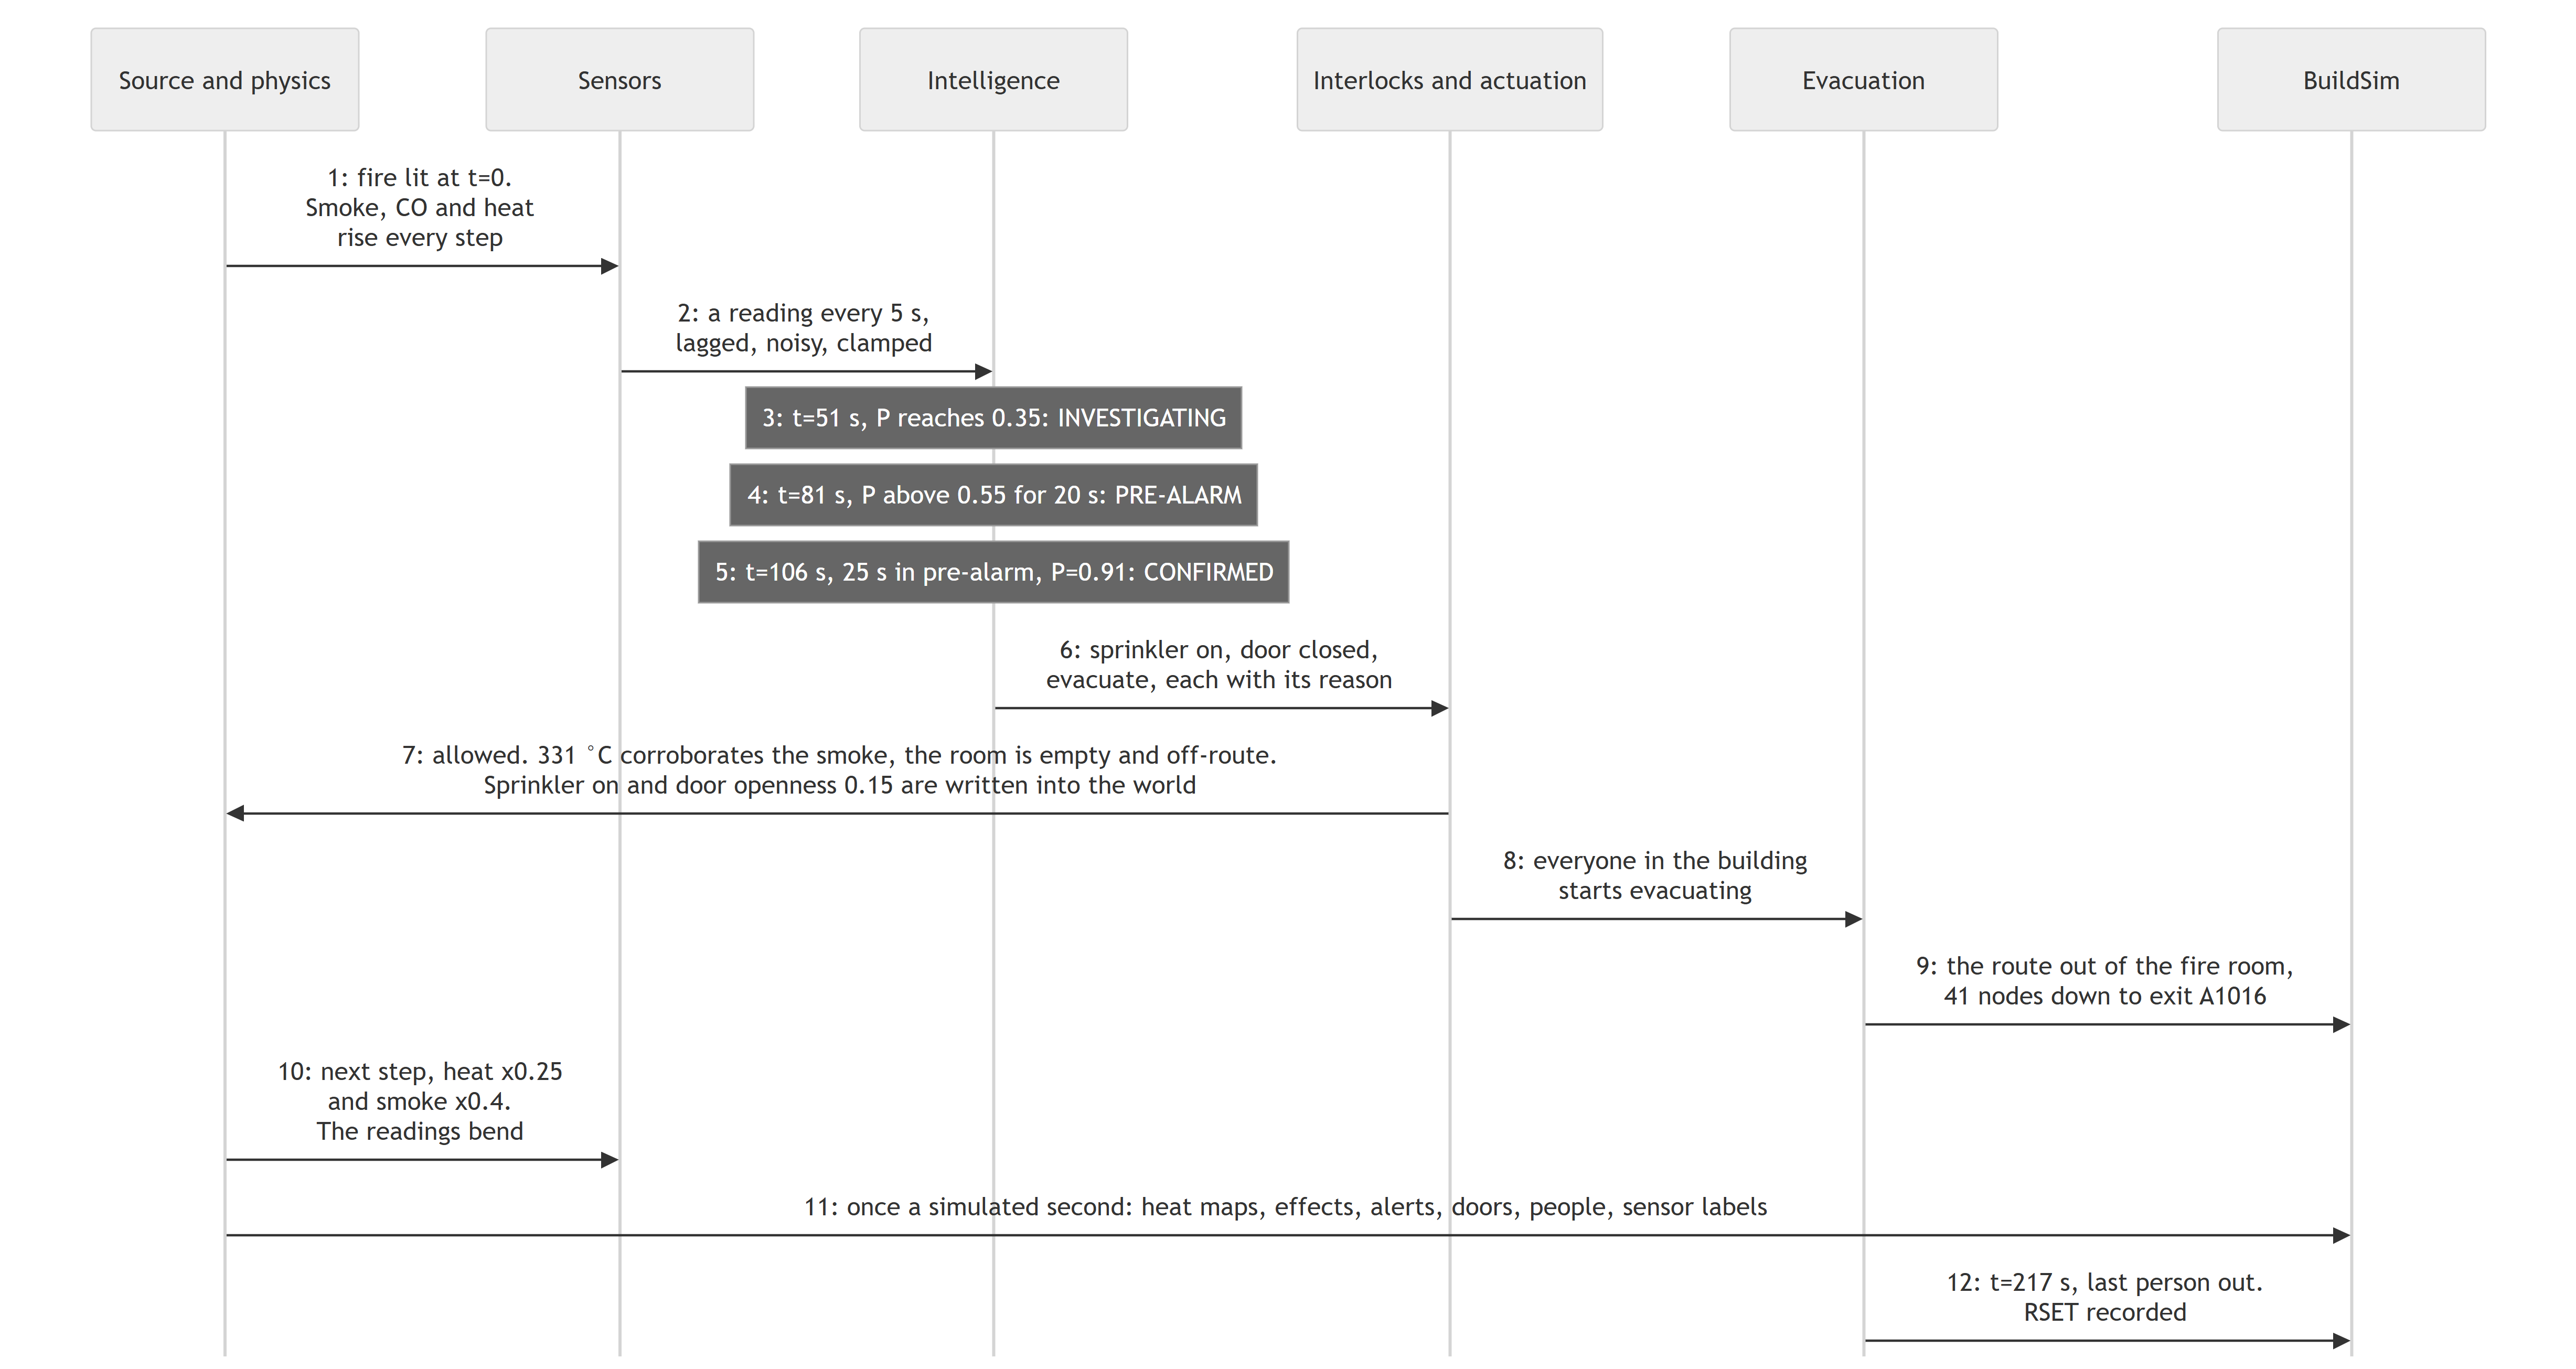
\includegraphics[width=1.00\linewidth]{images/dynamic.png}
\caption{C4 Dynamic diagram of the office fire, with the times measured in Section~11. Steps 3 to 5 are the dwells; step 7 is where the interlocks decide; step 10 is the loop closing.}
\label{fig:dynamic}
\end{figure}

Two things in the order matter. The response is issued and applied in the same
tick that confirms, so nothing waits for the next reading. And the fire door closed
only because A3505 happened to be empty and on nobody's route; had a student been
inside, step~7 would have refused the door, journalled why, and kept the request
pending until they left.

\subsection{8.2 Process lifecycle, state machine}

Every monitored room has one of these, and its transitions are the code in
\code{domain/agent.py}. The dwells are on the arrows.

\begin{figure}[H]
\centering
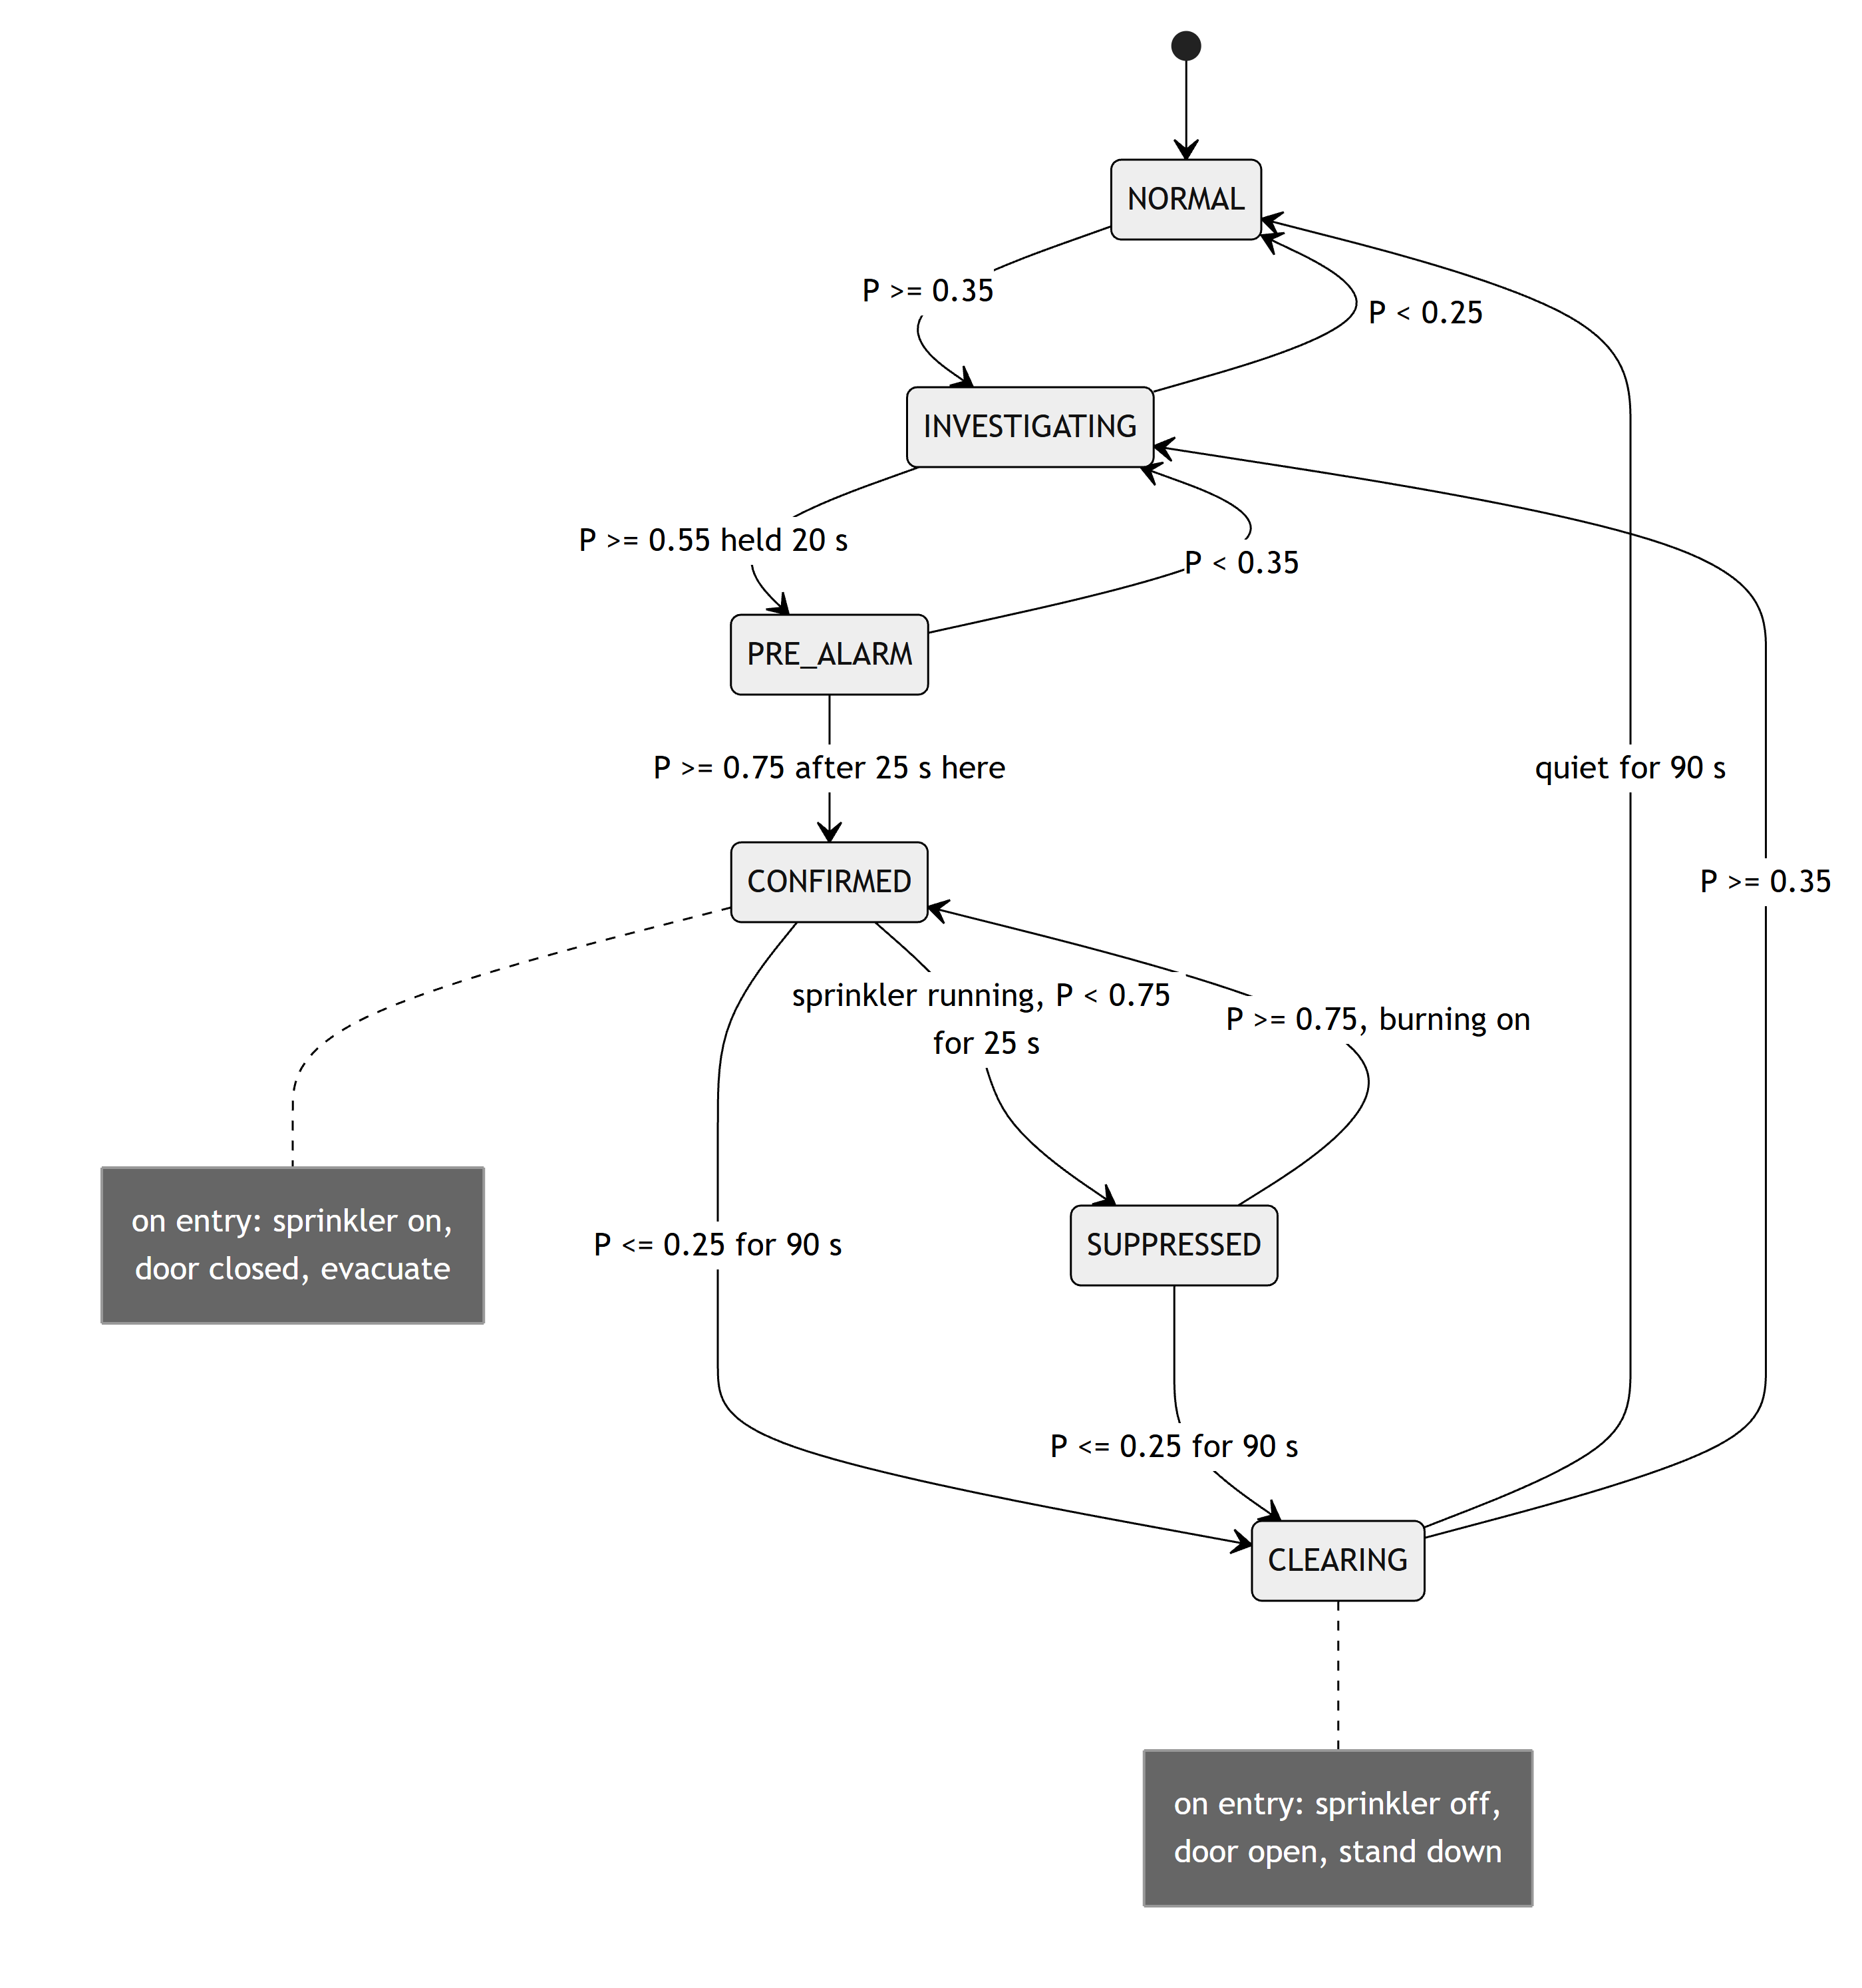
\includegraphics[width=0.72\linewidth]{images/state.png}
\caption{The per-room alarm state machine. Only two states ask for anything; every other arrow only changes what the room believes.}
\label{fig:state}
\end{figure}

\textsc{suppressed} is still an alarm: the fire is being held, not out, and the
confirmed state's outstanding requests stand. A fire that burns on through the
water climbs straight back to \textsc{confirmed}. Standing down needs the
probability to stay at or below 0.25 for 90\,s and then a further 90\,s of quiet
before the room stops being flagged as an incident, so a sensor that recovers for a
moment cannot reopen a door onto a fire. The process itself has a lifecycle of its
own outside this diagram: on startup the service loads the floors from BuildSim and
scatters the population; if BuildSim stops answering, the service marks itself
disconnected, keeps simulating, stops publishing, and waits for a reload rather
than crashing.
